A continuación, en esta sección se presentarán trabajos anteriores de investigación basados en la predicción de éxito o fracaso de campañas en Kickstarter o plataformas similares y el análisis de estas utilizando conjuntos de datos con estructuras similares al del presente trabajo. En cada uno se detalla el problema y su objetivo, la metodología implementada, las técnicas usadas y los resultados obtenidos.

\cite{pr_chen2013kickpredict} realizaron la publicación del reporte técnico \citetitle{pr_chen2013kickpredict} para el Departamento de Ciencias Computacionales y Matemáticas del Instituto de Tecnología de California, el cual traducido al español significa «KickPredict: Predicción del éxito de Kickstarter».

Ante la cantidad considerable de proyectos en Kickstarter que fracasaron en financiarse debido a los datos asignados por sus creadores, los autores desarrollaron un sistema predictivo de estado de financiamiento de un proyecto, el cual captura información en tiempo real y estima su resultado a partir de ello.

De acuerdo a la metodología seguida por los autores, el primer paso fue la recolección de datos de 20,000 proyectos completados, es decir, cuyo estado de financiamiento fue exitoso o fracasado. De esta cantidad, el 95\% fue destinado al subconjunto de entrenamiento. El siguiente paso fue el desarrollo de un algoritmo clasificador binario estándar para identificar las variables más importantes y generar el modelo de predicción. Para el sistema propuesto, se utilizaron Máquinas de Vectores de Soporte (SVM) entrenadas con cada combinatoria posible de las variables del conjunto de datos. Además de recolectar registros de proyectos, se complementó utilizando data de YouTube (determinar si un proyecto no utiliza videos de este medio en su descripción) y Twitter (número de veces en que el enlace del proyecto fue compartida) para enriquecer la investigación.

Las 4 variables más importantes encontradas del algoritmo clasificador fueron el número de proyectos patrocinados por el creador, número de proyectos creados por el creador, si presenta o no video, monto de la meta del proyecto. Evaluando el modelo con la métrica de exactitud, se alcanzó el valor de 0.90 al 40\% de transcurrida la duración de la campaña.

Finalmente, como último paso se implementó una aplicación en Android para la búsqueda de proyectos en Kickstarter y una extensión en Google Chrome para estimar el éxito y la exactitud de precisión de la predicción en tiempo real, mostrando la evolución de las cantidades patrocinadas en el tiempo transcurrido de la campaña, como se ilustra en la Figura \ref{2:fig111}.

\begin{figure}[!ht]
	\begin{center}
		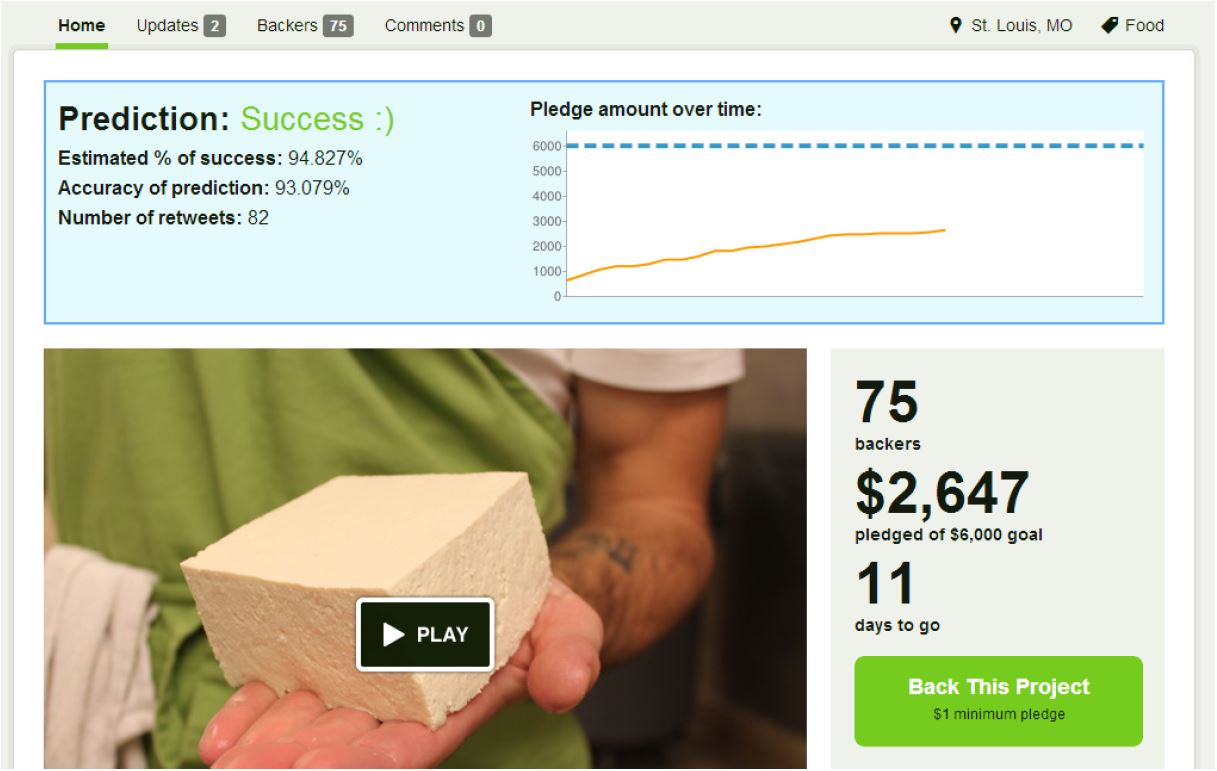
\includegraphics[width=0.7\textwidth]{2/figures/chen2013.jpg}
		\caption[Extensión de Google Chrome creada para predecir el estado del proyecto]{Extensión de Google Chrome creada para predecir el estado del proyecto.\\
			Fuente: \cite{pr_chen2013kickpredict}}
		\label{2:fig111}
	\end{center}
\end{figure}

En el acta de la conferencia «The 17th ACM conference on Computer supported cooperative work \& social computing (CSCW '14)», realizada del 15 al 19 de febrero del 2014 en Baltimore, Estados Unidos, \cite{pr_mitra2014phrases} publicaron el artículo titulado \citetitle{pr_mitra2014phrases}, el cual traducido al español significa «El lenguaje que hace que la gente dé: Frases que predicen el éxito en Kickstarter».

Debido a la existencia de poco conocimiento sobre los factores que impulsan a financiar proyectos a pesar del crecimiento en los últimos años de plataformas de financiamiento colectivo como Kickstarter, los autores elaboraron un modelo para predecir el éxito de financiamiento en proyectos crowdfunding a partir de frases textuales.

De acuerdo a la metodología seguida por los autores, el primer paso fue la recolección de 45,815 proyectos de Kickstarter del 2012. A continuación, se realizó limpieza de datos eliminando campañas inconclusas y con esto se procedió a extraer la información textual (descripción y recompensas del proyecto). El siguiente paso fue la generación del cuerpo de más de 9 millones de frases únicas, de las cuales quedaron 20,391 frases que aparecen al menos 50 veces en todos los proyectos. Finalmente, se creó un modelo de Regresión logística penalizada para proteger contra la colinealidad y escasez que prevalecen en el conjunto de datos de frases, de las cuales se pueda determinar cuáles son aquellas que ayudan que un proyecto sea financiado y cuáles lo contrario.

De las 59 variables de control que no son texto, 29 que tenían «valores aceptables» tenían pesos positivos. 15 variables fueron consideradas para proyectos que serán financiados, mientras que 14 para los que no. Se obtuvo un Top 100 de frases que tenían pesos positivos (proyectos que sí serán financiados), así como también para aquellas con pesos negativos (proyectos que no serán financiados) como se ilustra en la Figura \ref{2:fig112}. El ratio de error del modelo propuesto, considerando las variables de control más las frases, fue de 2.24\% frente al 17.03\% solo considerando las variables de control, y 48.47\% de la base comparada.

\begin{figure}[!ht]
	\centering
	\small
	\begin{subfigure}{.5\textwidth}
		\centering
		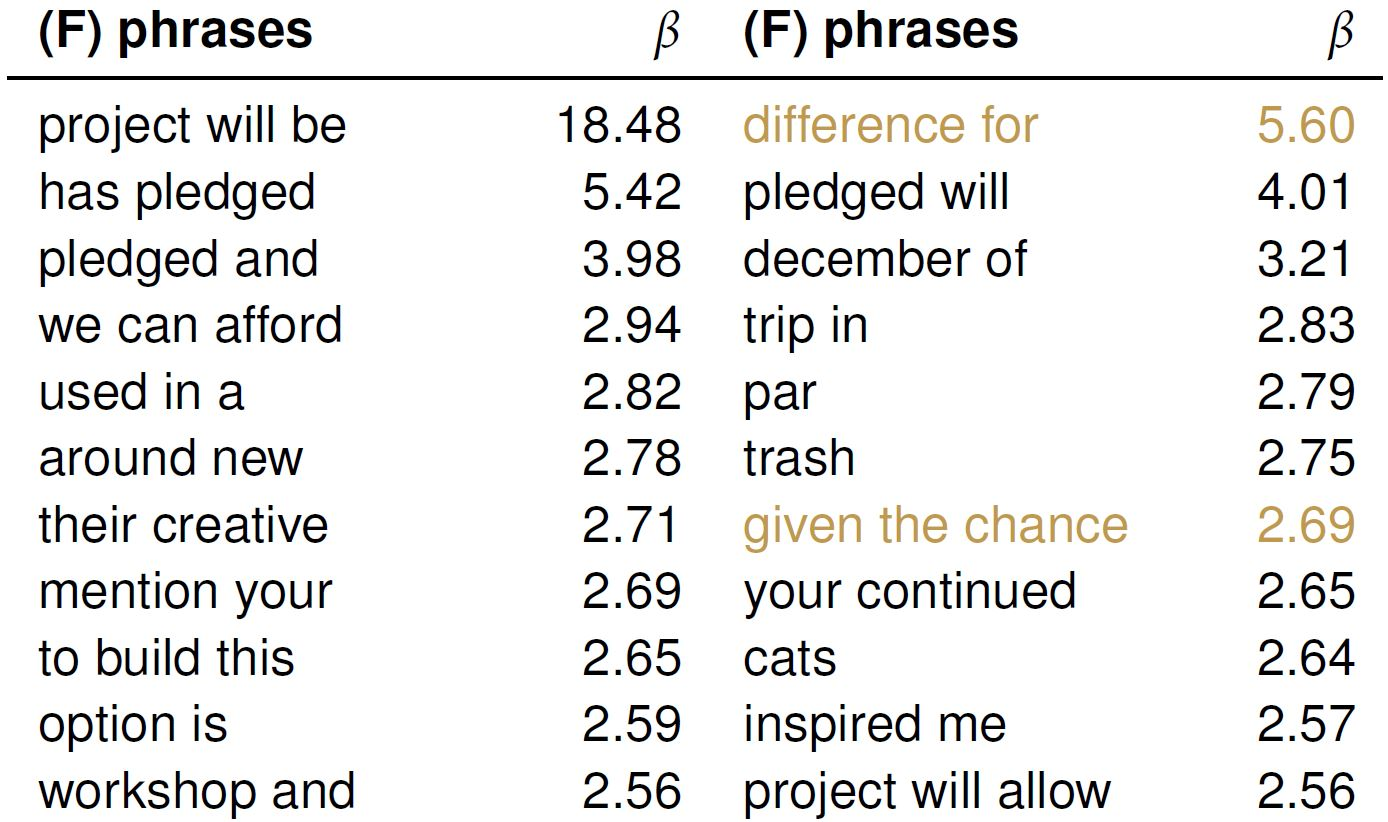
\includegraphics[width=0.85\linewidth]{2/figures/mitra2014_resultadoA.jpg}
		\caption{Frases para proyectos exitosos}
	\end{subfigure}%
	\begin{subfigure}{.5\textwidth}
		\centering
		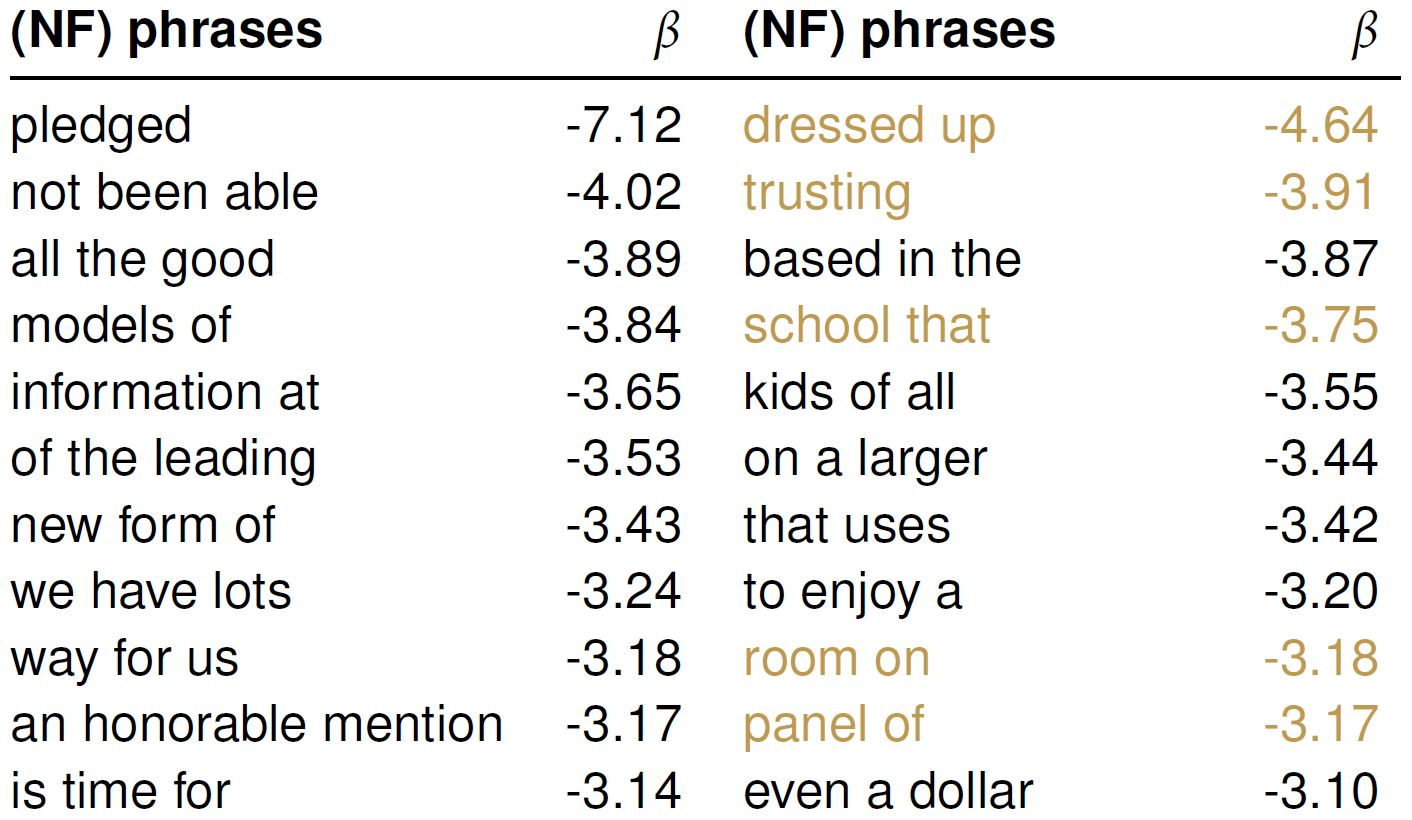
\includegraphics[width=0.85\linewidth]{2/figures/mitra2014_resultadoB.jpg}
		\caption{Frases para proyectos fracasados}
	\end{subfigure}
	\caption[Ejemplos de frases del Top 100 y sus respectivos pesos que señalan si un proyecto será o no financiado]{Ejemplos de frases del Top 100 y sus respectivos pesos que señalan si un proyecto será o no financiado.\\
		Fuente: \cite{pr_mitra2014phrases}}
	\label{2:fig112}
\end{figure}

En el acta de la conferencia «Twenty-first Americas Conference on Information Systems», realizada en Puerto Rico en el año 2015, \cite{pr_zhou2015projectdesc} publicaron el artículo titulado \citetitle{pr_zhou2015projectdesc}, el cual traducido al español significa «Money Talks: un modelo predictivo sobre el éxito del crowdfunding utilizando la descripción del proyecto».

Las investigaciones existentes de crowdfunding se centran principalmente en las variables básicas del proyecto como la categoría y la meta; sin embargo, hay muy pocos estudios basados en el contenido de la información, es decir, en la descripción del mismo. Por ello, el objetivo de los autores fue estudiar la influencia y el impacto del uso de descripciones de proyectos en su éxito de financiación para predecirlo.

De acuerdo a la metodología seguida por los autores, el primer paso fue la operacionalización de los constructos, es decir, cómo se consideraría la información recolectada a partir de los antecedentes en la literatura. A continuación, se recolectó información de más de 154 mil proyectos de Kickstarter entre 2009 y 2014. Luego, se desarrolló un modelo de Regresión Logística usando variables previamente identificadas como la meta del proyecto, duración del proyecto, si el creador presentaba conexión a Facebook, el número de sus amigos en Facebook, si el proyecto incluye una imagen, si el proyecto incluye un video, el número de recompensas, el año de lanzamiento del proyecto, y la categoría del proyecto. A éstas se añadieron el número de palabras en la descripción del proyecto, su legibilidad medido por Índice de niebla Gunning, ratio de positivo y negativo en descripción del proyecto, número de proyectos previamente creados y número de proyectos previamente patrocinados por el autor.

Finalmente, la propuesta se comparó contra otros modelos de la base y convencionales. Todos los modelos fueron evaluados por el valor-F probándose en validaciones cruzadas de 3, 5 y 10 iteraciones. Bajo esta métrica, el mejor modelo fue el propuesto, alcanzando un valor-F de 71.17 con 10 iteraciones. Asimismo, al ser comparado mediante la curva ROC, el modelo de los autores logró mejor performance frente al resto, superando el valor de 0.70 y alcanzando un ratio de verdaderos positivos frente al de falsos positivos como se aprecia en la Figura \ref{2:fig113}.

\begin{figure}[!ht]
	\begin{center}
		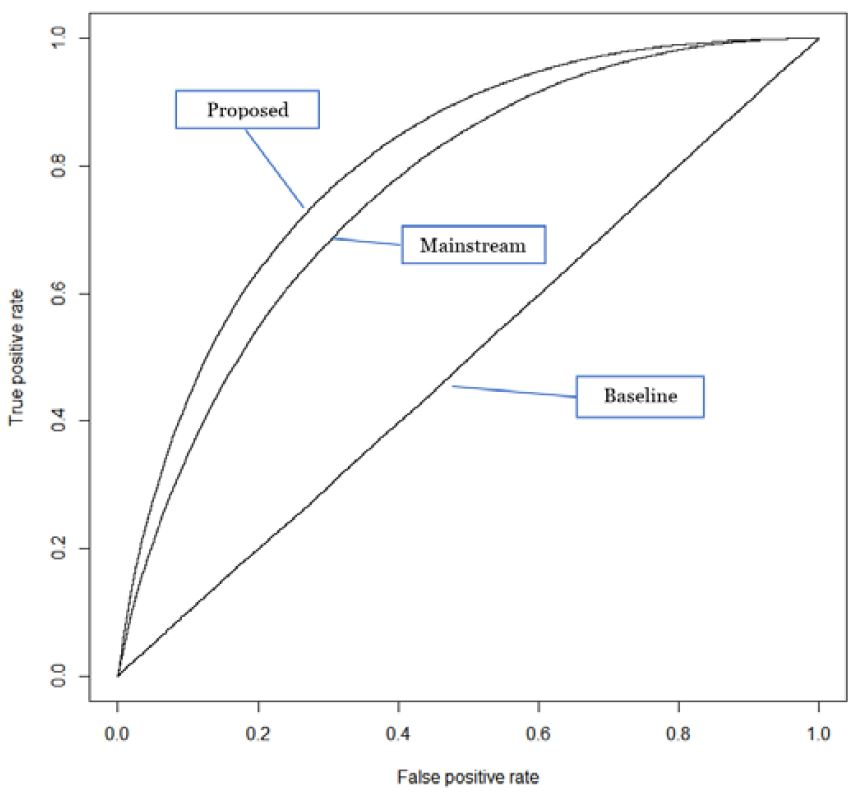
\includegraphics[width=0.50\textwidth]{2/figures/zhou2015.jpg}
		\caption[Curvas ROC del modelo propuesto, el de base y el convencional]{Curvas ROC del modelo propuesto de los autores, el de base y el convencional.\\
			Fuente: \cite{pr_zhou2015projectdesc}}
		\label{2:fig113}
	\end{center}
\end{figure}

En el acta de la conferencia «Pacific Asia Conference on Information Systems (PACIS) 2015» realizada en New York, Estados Unidos, en el año 2015, \cite{pr_chen2015predcrowd} publicaron el artículo titulado \citetitle{pr_chen2015predcrowd}, el cual traducido al español significa «¿Tu proyecto obtendrá la luz verda? Prediciendo el éxito de campañas de financiamiento colectivo».

Desde el surgimiento de campañas de financiamiento colectivo en sitios web así como estudios de estos casos, la mayoría de estos presentan problemas en la predicción de éxito de una campaña por distintas casuísticas ya que suelen enfocarse en aquellos concluídos. Ante la interrogante de la posibilidad de desarrollar una técnica efectiva para predecir si una campaña será exitosa o no en diferentes momentos de tiempo de las campañas de crowdfunding, los autores desarrollaron una técnica efectiva para predecir si una campaña de crowdfunding tendrá éxito o fracasará a través de extracción y posterior uso de características estáticas y dinámicas.

De acuerdo a la metodología seguida por los autores, el primer paso fue recolectar más de 4 mil proyectos de Kickstarter obtenido tanto directamente desde el sitio como con ayuda de la página web Kickspy, entre el primer y último día de abril del 2014. Después de realizado el pre-procesamiento, se extrajeron las características para la tarea de predicción de objetivos. Luego, estas características se clasificaron en 5 categorías: características intrínsecas, mecanismo financiero, calidad y sentimiento del contenido, interacción social y efecto de progresión, en donde las 3 primeras + interacción social corresponden a un nuevo grupo asignado como «características estáticas», mientras que la última + interacción social se asignó como «características dinámicas». Ambos nuevos conjuntos agrupados finalmente fueron entrenados en una serie de 8 modelos de Bosques Aleatorios para diferentes etapas (puntos de tiempo) de la campaña desde el día 0 hasta el día 7.

Finalmente, se comparó el modelo propuesto considerando todas sus características contra el mismo alternando versiones que solo usaron algunas y un trabajo previo de otro autor. El resultado final de la evaluación medidos por la exactitud determinó que el modelo propuesto considerando todas sus características logró la mejor performance, con un valor de 0.8467. Asimismo, como se observa en la Figura \ref{2:fig114}, se evaluaron campañas exitosas y fracasadas con la precisión, sensibilidad y puntaje F1 en distintas etapas de tiempo (7 primeros días), en donde se determinó que, a mayor tiempo transcurrido, mejores son sus resultados.

\begin{figure}[!ht]
	\begin{center}
		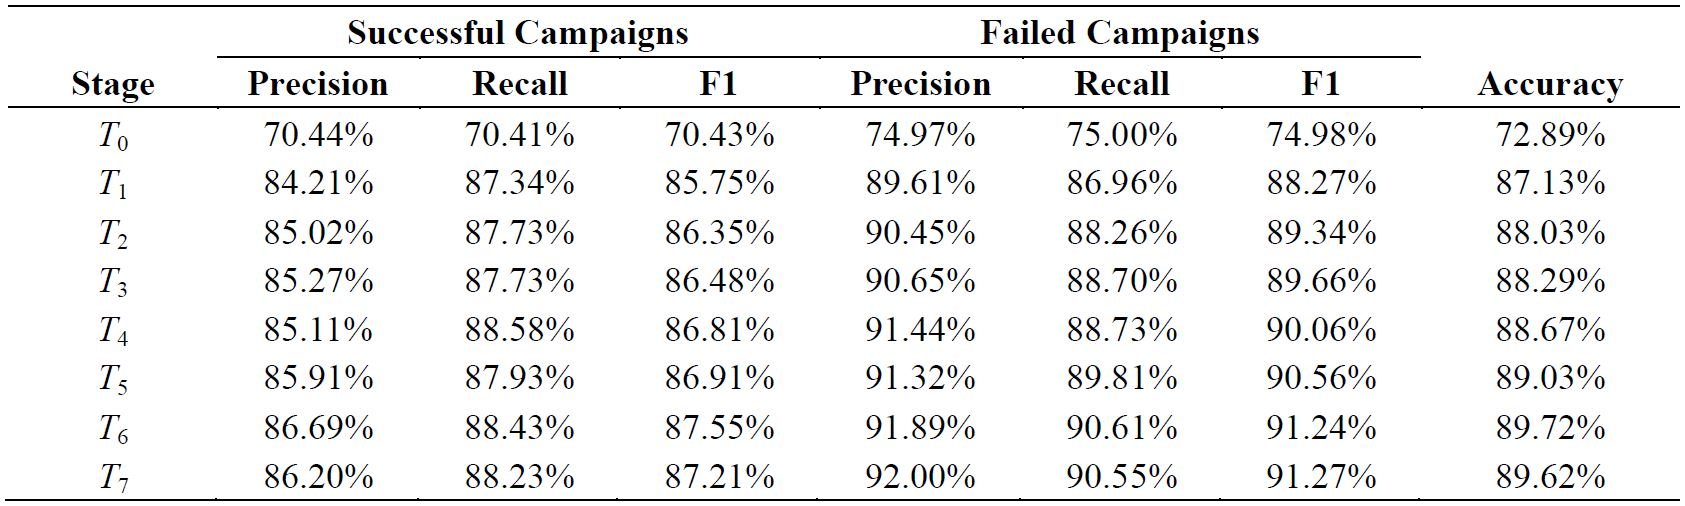
\includegraphics[width=0.90\textwidth]{2/figures/chen2015.jpg}
		\caption[Evaluación de la performance de los modelos construidos en distintas etapas de tiempo]{Evaluación de la performance de los modelos construidos en distintas etapas de tiempo.\\
			Fuente: \cite{pr_chen2015predcrowd}}
		\label{2:fig114}
	\end{center}
\end{figure}

\cite{pr_beckwith2016predcrowd} publicó la investigación de su tesis de grado titulada \citetitle{pr_beckwith2016predcrowd}, traducida al español como «Prediciendo el éxito en el financiamiento colectivo de acciones», para el programa académico «Joseph Wharton Scholars» de la Universidad de Pensilvania en el año 2016.

El financiamiento colectivo o crowdfunding de inversión se vuelve cada vez más popular. Este concepto permite que los emprendedores ofrezcan algún tipo de producto o servicio como compensación por contribuciones financieras una vez que ya se tengan ventas reales o acuerdos comerciales. Resulta ser muy interesante para los patrocinadores ya que no se necesita contar con un capital muy alto. A cambio, ellos recibirán algo a cambio una vez que el proyecto se realice. Este factor permite su mayor probabilidad de éxito de financiamiento al momento de darse una campaña de este tipo de crowdfunding ya que los patrocinadores pueden invertir en más de un proyecto a la vez. A partir de este punto, surge la interrogante por conocer los motivos de inversión y no inversión en ciertos start-ups ante la similitud de características observables. Por ello, el objetivo del autor fue determinar la relación entre las características de una compañía determinada y su capacidad para recaudar fondos en la plataforma de financiamiento colectivo de capital AngelList.

De acuerdo a la metodología seguida por el autor, el primer paso fue la recolección de más de 5 mil compañías de AngelList que solicitaron contribuciones financieras. De esta cantidad, se consideraron aquellas con datos completos (2,603 empresas). Luego del pre-procesamiento del conjunto final de datos, el investigador desarrolló un modelo de Regresión logística usando las siguientes variables: si la empresa previamente había recibido o no financiación, si la compañía cuenta con perfil en Twitter, número de veces que la compañía había sido mencionada en alguna publicación, número de veces que la compañía había sido mencionada en TechCrunch, número de personas listadas como co-fundadoras en el perfil de la compañía AngelList, si AngelList lista entre 11 y 50 empleados como tamaño de la empresa, si la compañía está ubicada en San Francisco, si entre los fundadores de AngelList al menos uno de ellos cuenta con un MBA, si entre los fundadores de AngelList al menos uno de ellos realizó sus estudios en alguna de las mejores 20 universidades de Estados Unidos, y el número de cierre del S\&P 500 el día anterior al lanzamiento de la campaña de crowdfunding de AngelList. La propuesta fue comparada con un Árbol de Decisión CART, un modelo de Naïve Bayes y una Máquina de Vectores de Soporte. Finalmente, se evaluó el modelo propuesto mediante la exactitud, precisión, sensibilidad, puntaje F1, y área bajo la curva (AUC).

Bajo las métricas mencionadas, el modelo del autor superó a los otros 3 modelos comparados en cada una de ellas. Sus resultados fueron 0.87 de exactitud, precisión promedio de 0.85, sensibilidad promedio de 0.88, puntaje F1 promedio de 0.86, y área bajo la curva de 0.74, este último como se observa en la Figura \ref{2:fig115}.

\begin{figure}[!ht]
	\begin{center}
		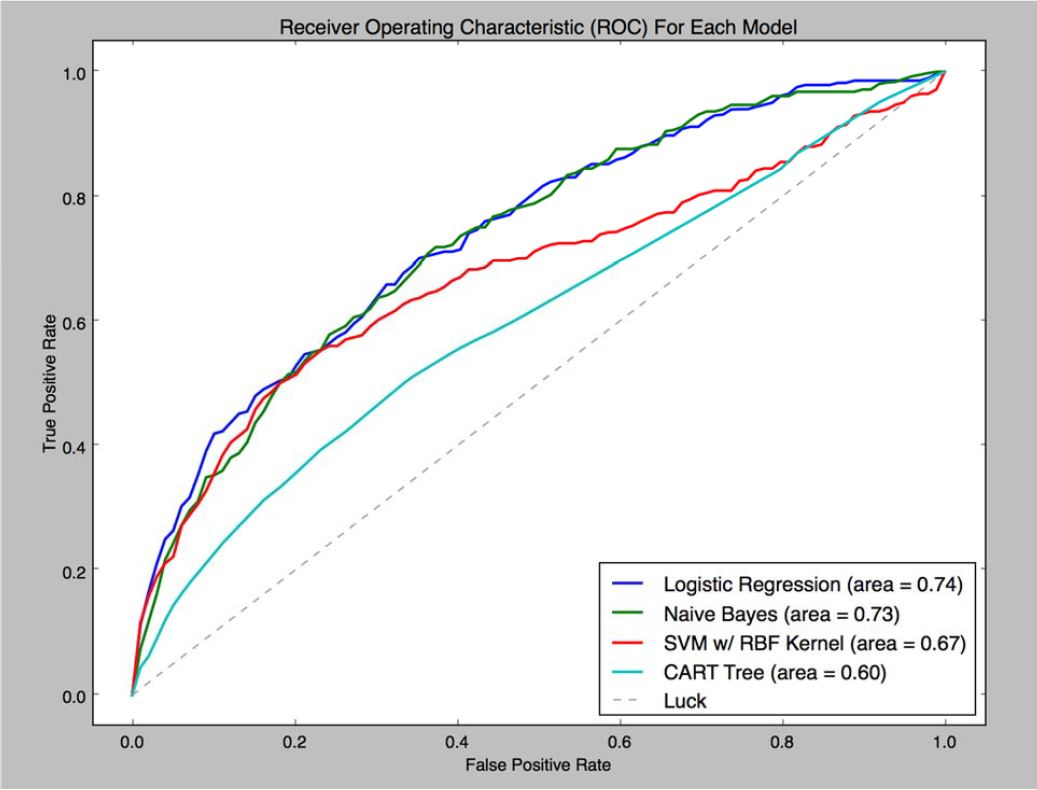
\includegraphics[width=0.70\textwidth]{2/figures/beckwith2016.jpg}
		\caption[Curva ROC para cada modelo utilizado por el autor]{Curva ROC para cada modelo utilizado por el autor.\\
		Fuente: \cite{pr_beckwith2016predcrowd}}
		\label{2:fig115}
	\end{center}
\end{figure}

En el acta de la conferencia «The Ninth ACM International Conference on Web Search and Data Mining (WSDM’ 16)» realizado en San Francisco, Estados Unidos, en el año 2016, \cite{pr_li2016predcrowd} publicaron el artículo titulado \citetitle{pr_li2016predcrowd}, el cual traducido al español significa «Predicción de éxito de un proyecto en ambientes de financiamiento colectivo».

Durante la última década se han elaborado una serie de modelos de clasificación que permitan pronosticar con cierto nivel de exactitud si algunos proyectos de financiamiento colectivo tendrán éxito o no. Sin embargo, el hecho de estimar si esto ocurrirá durante el plazo dado de la campaña no puede proporcionar una guía adecuada a los patrocinadores que desean invertir en proyectos populares. Es entonces que se cuestiona la posibilidad de predecir el éxito de campañas en sitios web de crowdfunding como Kickstarter considerando características obtenidas durante la operación de la campaña. Para resolver esta interrogante, los autores formularon la predicción del éxito del proyecto como un problema de análisis de supervivencia y aplicar el enfoque de regresión censurada.

De acuerdo a la metodología seguida por los autores, el primer paso fue la recolección de más de 27 mil proyectos de Kickstarter entre diciembre del 2013 y junio del 2014 para la data estática, a los cuales se removieron aquellos que fueron cancelados, suspendidos o con menos de 1 patrocinador y monto prometido de \$100. Asimismo, para la data dinámica se capturaron más de 106 mil tweets de Twitter que contenían el enlace rápido hacia la página de Kickstarter. Una vez obtenidos los conjuntos de datos, se realizó el pre-procesamiento. A continuación, se elaboraron 2 modelos predictivos para evaluar la regresión censurada: 1 modelo de distribución logística y 1 de distribución log-logística. Para poder compararlos, se elaboraron adicionalmente otros métodos para manejar observaciones censuradas, mencionados en la literatura como Cox, Regresión Tobit, estimación Buckley-James e Índice de Concordancia Boosting (BoostCI).

Finalmente, como resultado de las múltiples pruebas en los modelos, en los cuales se experimentaron distintas combinatorias con la data estática y dinámica, así como agregando y desagregando proyectos fracasados, se concluyó que el modelo de Regresión log-logística evaluado con el área bajo la curva (AUC) presentó mejor performance que el resto en 3 de las 4 combinatorias, alcanzando su mejor nivel en el conjunto de datos que combina data estática, dinámica, de características de proyectos transcurridos los primeros 3 días y con proyectos fracasados, con un puntaje Survival AUC de 0.9030, como se representa en la Figura \ref{2:fig116}.

\begin{figure}[!ht]
	\begin{center}
		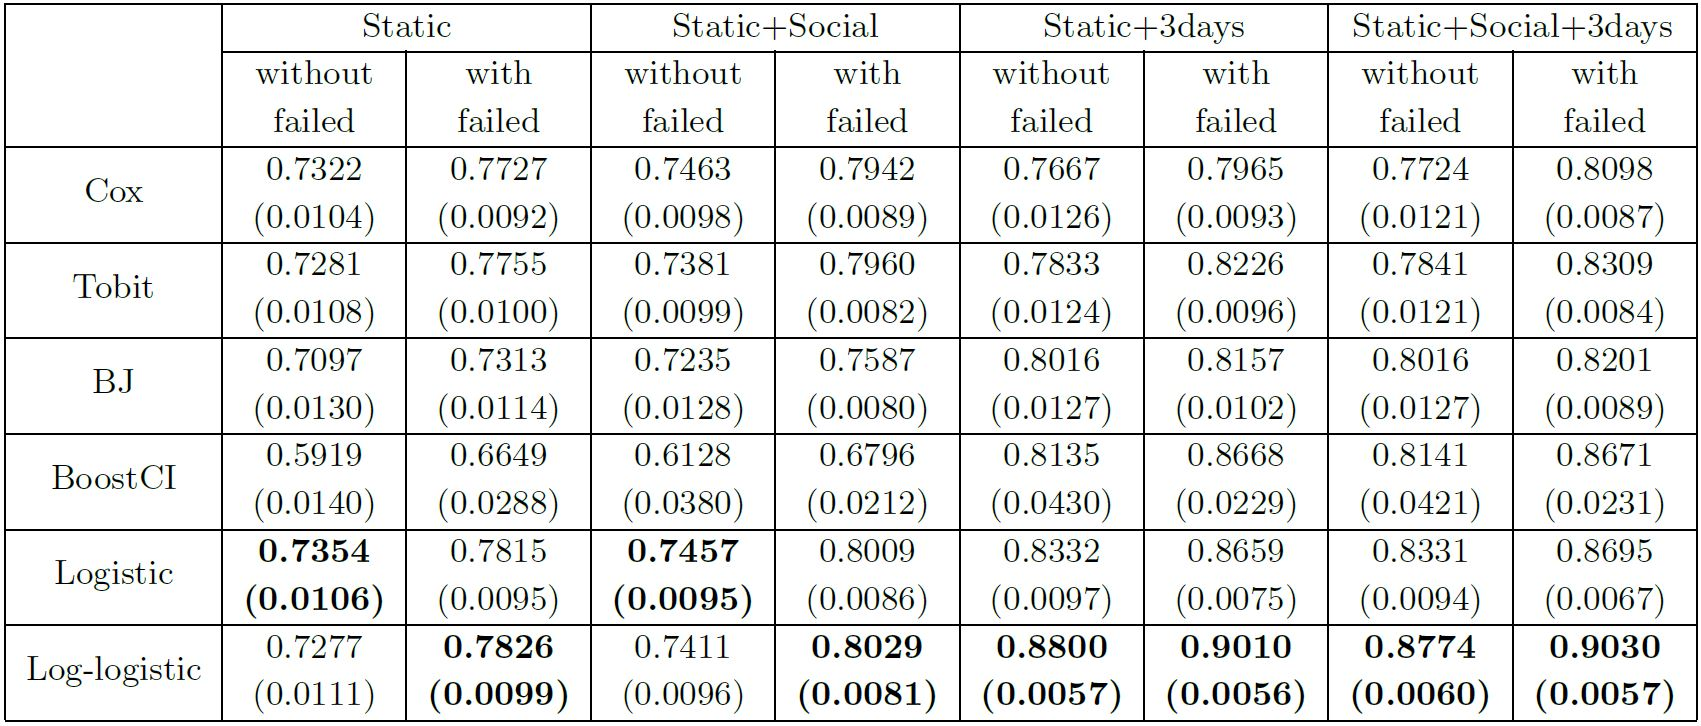
\includegraphics[width=0.85\textwidth]{2/figures/li2016.jpg}
		\caption[Comparación de resultados de conjuntos de datos de distintas características de proyectos considerando incluir o no proyectos fracasados]{Comparación de resultados de conjuntos de datos de distintas características de proyectos considerando incluir o no proyectos fracasados.\\
			Fuente: \cite{pr_li2016predcrowd}}
		\label{2:fig116}
	\end{center}
\end{figure}

\cite{pr_yuan2016textanalytics} publicaron un artículo en la revista «Decision Support Systems», en el año 2016, titulado \citetitle{pr_yuan2016textanalytics}, el cual traducido al español significa «Los determinantes del éxito del financiamiento colectivo: Un enfoque de analítica semántica de texto».

Actualmente existen diversos estudios de éxito de campañas de financiamiento colectivo, la mayoría usando modelos predictivos en proyectos crowdfunding basados en recompensas y análisis de características poco profundas del lenguaje en descripción de los proyectos (por ejemplo, número de palabras, errores ortográficos, etc) así como en la implementación de métodos de Aprendizaje Automático. Como propuesta alterna, los autores construyeron un marco de trabajo basado en análisis de texto que pueda extraer semánticas de descripciones textuales de proyectos para predecir sus resultados de recaudación de fondos.

De acuerdo a la metodología seguida por los autores, el primer paso consistió en recolectar 500 proyectos de 2 webs chinas sobre crowdfunding cada una. Luego, se construyó el marco de trabajo del análisis textual ilustrado en la Figura \ref{2:fig117}. A continuación, se diseñó un modelo de Bosque Aleatorio para los datos numéricos, y POS Tag Stemming más modelo DC-LDA más características tópicas para los datos textuales con la finalidad de realizar una extracción más efectiva de las características tópicas a partir de las descripciones. Esta arquitectura se comparó con otros modelos en la literatura de la publicación. Luego, se realizó un análisis empírico para identificar características discriminatorias que influye en el éxito de la recaudación de fondos.

\begin{figure}[!ht]
	\begin{center}
		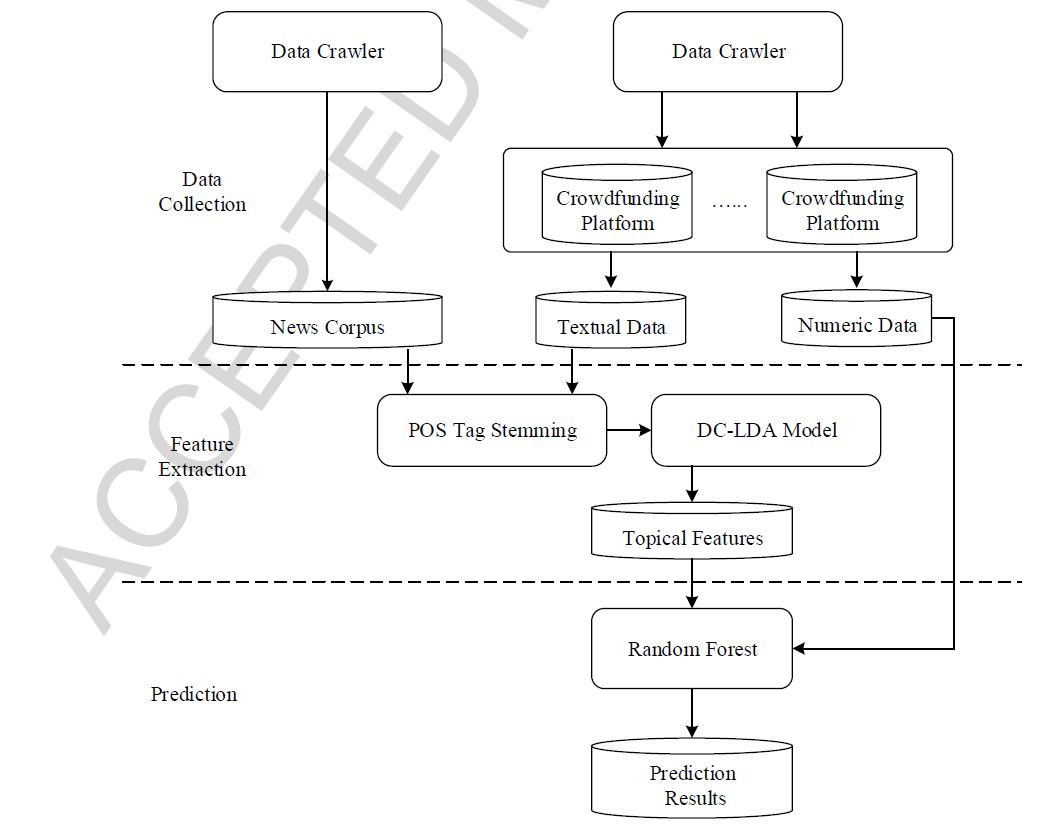
\includegraphics[width=0.62\textwidth]{2/figures/yuan2016a.jpg}
		\caption[Marco de trabajo de analítica textual de los autores]{Marco de trabajo de analítica textual de los autores.\\
			Fuente: \cite{pr_yuan2016textanalytics}}
		\label{2:fig117}
	\end{center}
\end{figure}

Finalmente, se evaluaron ambos conjuntos de datos. Para los datos numéricos, la mejor performance se obtuvo evaluando el modelo con la sensibilidad para el Bosque Aleatorio (0.98 en la segunda data); mientras que para los datos textuales, el modelo DC-LDA (al ser comparado con el LDA normal) obtuvo un puntaje F1 de 0.91 como se observa en la Figura \ref{2:fig118}.

\begin{figure}[!ht]
	\begin{center}
		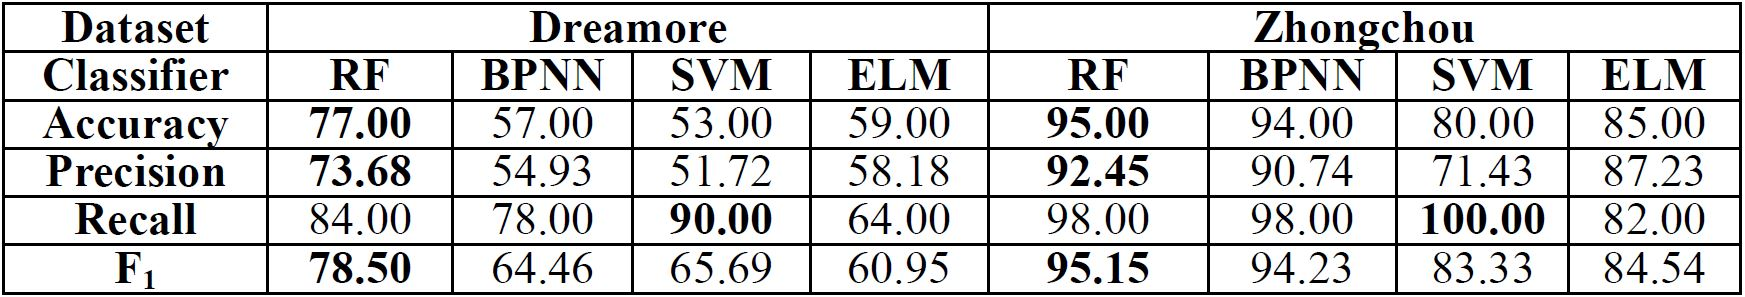
\includegraphics[width=0.85\textwidth]{2/figures/yuan2016b.jpg}
		\caption[Performance de ambas bases de datos con distintas métricas]{Performance de ambas bases de datos con distintas métricas.\\
			Fuente: \cite{pr_yuan2016textanalytics}}
		\label{2:fig118}
	\end{center}
\end{figure}

\subsection{Using Language to Predict Kickstarter Success \citep*{pr_sawhney2016usingLT}}
\citeauthor{pr_sawhney2016usingLT} realizaron la publicación «Using Language to Predict Kickstarter Success» para el Departamento de Ciencia de la Computación de la Universidad Standford. Este fue titulado \citetitle{pr_sawhney2016usingLT} la cual traducida al español significa «Uso del lenguaje para predecir el éxito de Kickstarter».

\subsubsection{Planteamiento del Problema y objetivo}
Dada la considerable cantidad de investigaciones y trabajos de predicción de éxito financiamiento de proyectos basados en la evolución de variables estáticas, los autores construyeron un clasificador binario que logre predecir el éxito de una campaña a partir de su contenido, características lingüísticas y metadata.

\subsubsection{Técnicas empleadas por los autores}
Los autores utilizaron el Clasificador de Naive Bayes para las características primarias, Parts-of-Speech Tagging (POS), legibilidad Flesch-Kincaid, y Máquina de Vectores de Soporte (SVM) para los conjuntos de entrenamiento y prueba.

\subsubsection{Metodología empleada por los autores}
Se recolectaron más de 160 mil proyectos de Kickstarter, separando en proporciones de 0.80/0.20 los subconjuntos de entrenamiento y prueba respectivamente. A continuación, recopilaron las características primarias y se realizó un análisis de sentimientos. Luego, asignaron las meta-características para utilizarlos como entradas durante el entrenamiento de los modelos. Finalmente, estos últimos fueron calibrados y se probaron con el subconjunto de prueba para finalmente ser evaluados.

\subsubsection{Resultados obtenidos}
Considerando el modelo solo con las características primarias, el nivel de exactitud alcanzó 0.65. Sin embargo, utilizando el clasificador entrenado con SVM, el valor de la exactitud logró llegar hasta 0.92.

\subsection{Effect of Social Media Connectivity on Success of Crowdfunding Campaigns \citep*{pr_kaur2017socmedcrowd}}
\citeauthor{pr_kaur2017socmedcrowd} realizaron un artículo de investigación el cual fue publicado en la revista «Procedia Computer Science» en el año 2017. Este fue titulado \citetitle{pr_kaur2017socmedcrowd} la cual traducida al español significa «Efecto de conectividad en medios sociales en éxito de campañas de financiamiento colectivo».

\subsubsection{Planteamiento del Problema y objetivo}
Los proyectos de crowdfunding, así como los proyectos lanzados en sitios dedicados a esto, han crecido exponencialmente en los últimos años. Los medios sociales desempeñan un papel importante en la difusión de palabras sobre una campaña y en la obtención de fondos con éxito. Después de lanzarse una campaña, su éxito se define por la interacción social de los creadores en la plataforma y en las redes sociales. Además, el tamaño de la red social del creador y su presencia en línea motiva a los patrocinadores a participar y financiar el proyecto. Partiendo de esta premisa, se busca conocer el impacto de la conectividad con las redes sociales y las interacciones sociales en el rendimiento del crowdfunding.

Para ello, los autores plantearon el desarrollo de un modelo predictivo que comprenda las características de la campaña y sumado a eso, la información sobre la conectividad con las diversas redes sociales como Facebook y Twitter.

\subsubsection{Técnicas empleadas por los autores}
Los autores propusieron un modelo de Regresión Logística, el cual compararon con algunos enunciados en sus antecedentes como Naïve Bayes, J48 y Bosques Aleatorios.

\subsubsection{Metodología empleada por los autores}
Se recolectaron 2 tipos de conjuntos de datos: el primero obtenido desde Kickstarter en el mes de Abril del 2014, con más de 4 mil campañas; mientras que el segundo a través del perfil del creador vinculado a redes sociales. El primer conjunto comprendió las variables de categoría, tipo de divisa, monto de la meta, monto prometido, número de recompensas, duración de la campaña en días, y el estado final de financiamiento (exitoso o fracasado). Por el lado del segundo conjunto, además de obtener marcas de hacia qué redes sociales el creador se conecta, mediante el enlace se extrajeron más de 19 mil tweets en el que se promocionaron las campañas gracias a la API de Twitter.

Una vez armados los conjuntos de datos, se creó el modelo propuesto y se comparó con las bases de referencia usando como métrica principal la exactitud. Previo a este paso, todas las variables consideradas se evaluaron en una matriz de correlaciones con el valor de “exitoso” de la variable dependiente.

\subsubsection{Resultados obtenidos}
Culminados los experimentos de la selección de variables en la matriz de correlaciones, así como la ejecución del modelo de Regresión Logística, la exactitud de este alcanzó un valor de 0.767 para un subconjunto de 66\% de entrenamiento y de 34\% de prueba, indicando así que la conectividad a medios sociales e interacciones en ellos influye en la predicción de éxito de la campaña. Asimismo, evaluando también con precisión y sensibilidad promedio, el ratio alcanzó 0.768 y 0.767 respectivamente.

\subsection{Supervised Learning Model For Kickstarter Campaigns With R Mining \citep*{pr_kamath2018suplearn}}
\citeauthor{pr_kamath2018suplearn} realizaron un artículo de investigación el cual fue publicado en la revista «International Journal of Information Technology, Modeling and Computing» en el año 2018. Este fue titulado \citetitle{pr_kamath2018suplearn} la cual traducida al español significa «Modelo de aprendizaje supervisado para campañas de Kickstarter con R Mining».

\subsubsection{Planteamiento del Problema y objetivo}
Kickstarter actualmente es la plataforma web basado en crowdfunding más grande existente. Sin embargo, no todas las campañas que se encuentran en su portal son exitosas. Algunos trabajos previos citados en este artículo citan que el lenguaje usado en las campañas alcanza el poder predictivo de 58.86\%, es decir, la descripción semántica de un proyecto ayuda considerablemente en la predicción de éxito debido a que muchos patrocinadores se fijan en la calidad presente en una campaña antes de invertir.  Sin embargo, es dejada de lado en muchos trabajos de investigación destinados a la predicción de éxito de financiamiento, así como también las interacciones de un proyecto en redes sociales. Para el tiempo en que este artículo fue publicado, el nivel de exactitud de los modelos predictivos ya existentes bordeaba por el 68\% como el descrito anteriormente

Ante esto, autores desarrollaron un sistema con técnicas de Aprendizaje Automático usando el entorno R aplicada a conjunto de datos de campañas en Kickstarter para clasificar proyectos entrenando diferentes clasificadores en esta data y predecir con un alto nivel de exactitud.

\subsubsection{Técnicas empleadas por los autores}
Los autores elaboraron 5 modelos clasificadores para la investigación: Árbol de decisión, Bosque Aleatorio, Red Neuronal Artificial, Vecino K más cercano, y Naïve Bayes. Se consideraron como variables para estos modelos al nombre del proyecto, URL del proyecto, descripción del proyecto, categoría, sub-categoría, número de patrocinadores, monto total patrocinado, meta de financiación, fecha de lanzamiento del proyecto, duración del proyecto, número de actualizaciones, número de recompensas, si el proyecto cuenta con video, localización del proyecto, y creador del proyecto.

\subsubsection{Metodología empleada por los autores}
En primer lugar, se analizó y definió el problema. A continuación, se recolectaron 120 proyectos de Kickstarter a través de su URL. Luego, las variables categóricas fueron transformadas en numéricas como parte del pre-procesamiento. Esto permitió realizar extracción y exploración del conjunto final mediante estadísticas descriptivas con paquetes de R. Una vez analizado los datos, se procedió a elaborar los modelos clasificadores y finalmente, con la matriz de confusión, se seleccionó el mejor de ellos evaluándolos mediante la exactitud.

\subsubsection{Resultados obtenidos}
Bajo la métrica de exactitud, el mejor de los 5 modelos clasificadores construidos fue la Red Neuronal, con un valor de 0.94.

\subsection{Prediction of Crowdfunding Project Success with Deep Learning \citep*{pr_yu2018deeplearning}}
\citeauthor{pr_yu2018deeplearning} realizaron un resumen de la conferencia «2018 IEEE 15th International Conference on e-Business Engineering (ICEBE)» del 12 al 14 de octubre del 2018 en Xi'an, China. Este fue titulado \citetitle{pr_yu2018deeplearning}, la cual traducida al español significa «Predicción del éxito de proyecto de financiamiento colectivo con Aprendizaje Profundo».

\subsubsection{Planteamiento del Problema y objetivo}
Debido al aumento dramático de la actividad de financiamiento colectivo en los últimos años, en el cual tanto creadores como patrocinadores participan, son más las campañas que buscan alcanzar su objetivo. Sin embargo, según el análisis empírico, solo la tercera parte lo logra. La incógnita que rodea a esta situación es la posibilidad de elaborar un modelo predictivo de éxito en proyectos de Kickstarter utilizando distintas técnicas al Aprendizaje Automático.

Por ello, los autores plantean como objetivo el desarrollo de un modelo que prediga el éxito del proyecto de crowdfunding con Aprendizaje Profundo usando registros históricos de campañas en Kickstarter.

\subsubsection{Técnicas empleadas por los autores}
Los autores elaboraron un modelo basado en un Perceptrón Multicapa (MLP), alimentado por 6 variables visibles de la campaña (metadata). Además, sus resultados se compararon con otros modelos considerados en sus antecentes como Bosques aleatorios, AdaBoost, Máquina de vectores de soporte, Árboles de decisión, Regresión logística y Naïve Bayes.

\subsubsection{Metodología empleada por los autores}
Se recolectaron más de 378 mil campañas de Kickstarter entre Mayo 2009 y Marzo 2018, recopilados retrospectivamente desde Kaggle. A continuación, realizaron análisis exploratorio de los datos para entender la data y seleccionar variables, y finalmente construyeron un modelo, el cual se comparó sus resultados con los de otros modelos.

\subsubsection{Resultados obtenidos}
Para comparar los resultados del modelo propuesto con los antecedentes, se tomaron en cuenta como métricas la exactitud y el área bajo la curva (AUC). De acuerdo a ellas, para ambos escenarios se lograron mejor performance, con una exactitud de 0.9320 y un área bajo la curva de 0.9323 frente al mejor modelo de los antecedentes, Bosques Aleatorios, que obtuvo como resultados 0.9293 y 0.9272 para las mismas métricas respectivamente.

\subsection{Content-based Success Prediction of Crowdfunding Campaigns: A Deep Learning Approach \citep*{pr_lee2018contentDL}}
\citeauthor{pr_lee2018contentDL} realizaron un resumen de la conferencia «Companion of the 2018 ACM Conference on Computer Supported Cooperative Work and Social Computing» del 3 al 7 de noviembre del 2018 en Jersey City, Estados Unidos. Este fue titulado \citetitle{pr_lee2018contentDL} la cual traducida al español significa «Predicción de éxito basada en contenido de campañas de crowdfunding: un enfoque de Aprendizaje Profundo».

\subsubsection{Planteamiento del Problema y objetivo}
El ratio promedio de éxito de financiamiento colectivo ha ido decreciendo en los últimos años a pesar del éxito de plataformas basadas en este tipo de apoyo a proyectos. Asimismo, los desafíos más relevantes fueron descubrir las razones de su éxito y lograr predecirlo.

Los autores plantearon utilizar solo el contenido textual de los proyectos (descripción de campaña, actualizaciones, comentarios y palabras obtenidas del video principal) para predecir el estado de financiamiento de proyectos de Tecnología (la categoría con ratio más bajo de éxito de financiamiento y a la vez, con los mayores montos financiados en la plataforma) a través de la creación de una Red Neuronal Profunda.

\subsubsection{Técnicas empleadas por los autores}
Se diseñó 1 Modelo de Secuencia a Secuencia (Seq2seq) con atención a nivel de oración y 1 Modelo de Atención Jerárquica (HAN).

\subsubsection{Metodología empleada por los autores}
Se recolectaron 216,136 proyectos de crowdfunding en Kickstarter, lanzados entre abril del 2009 y agosto del 2017. De ellos, se filtraron aquellos de la categoría Tecnología (22,982) para luego separar el conjunto de datos final en 0.80 (entrenamiento), 0.10 (validación) y 0.1 (prueba). Posteriormente, se diseñaron los 2 modelos de NLP, fueron entrenados y se compararon los resultados.

\subsubsection{Resultados obtenidos}
Ambos modelos fueron evaluados bajo la métrica de exactitud, bajo enfoques de distintos experimentos que alternaban la presencia de las variables. De todos ellos, basado en aquellos que utilizaron todas juntas, el modelo de Seq2seq + atención logró una exactitud de 0.80, mientras que el modelo HAN alcanzó el valor de 0.60.

\subsection{Estimating the Days to Success of Campaigns in Crowdfunding: A Deep Survival Perspective \citep*{pr_jin2019dayssuccess}}
\citeauthor{pr_jin2019dayssuccess} realizaron un resumen de la conferencia «The 33rd AAAI Conference on Artificial Intelligence (AAAI'2019)» del 27 de enero al 1 de febrero del 2019 en Honolulu, Hawái. Este fue titulado \citetitle{pr_jin2019dayssuccess} la cual traducida al español significa «Estimación de días de éxito de campañas en financiamiento colectivo: Una perspectiva de supervivencia profunda».

\subsubsection{Planteamiento del Problema y objetivo}
Dado el incremento de actividad en campañas de crowdfunding en sitios como Kickstarter o Indiegogo, los estudios sobre este tema también han ido de la mano. Sin embargo, la mayoría de investigaciones se enfocan en predecir el ratio de éxito de financiamiento en una campaña. El reto de predecir el tiempo de duración es más complicado porque se ve afectada por la variabilidad de la metadata y los comentarios del proyecto, resultando un alto nivel de fracaso (60\%) en la financiación de proyectos.

Los autores plantean la predicción de la fecha exacta de finalización de una campaña, así como controlar la distribución de patrocinios conforme a la evolución del tiempo.

\subsubsection{Técnicas empleadas por los autores}
Se elaboró un modelo Seq2seq (encoder + decoder) con previos multifacéticos (SMP) para la distribución de patrocinios y el tiempo de éxito, así como también un modelo evolutivo lineal para mantener el cambio de las distribuciones de patrocinios.

\subsubsection{Metodología empleada por los autores}
Se recolectó más de 14 mil proyectos de Indiegogo con información estática (descripción de campaña, descripción de las recompensas, categoría de la campaña, tipo del creador, duración declarada de financiación, meta declarada prometida, número de recompensas, precio máximo/mínimo/promedio de recompensas, plazo máximo/mínimo/promedio de entrega) y dinámica (comentarios), luego se definió el problema estudiado. A continuación, se introdujo los detalles técnicos de SMP, el conjunto pre-procesado de entrada, la arquitectura SMP, los previos multifacéticos y por último, el método de entrenamiento del modelo.

\subsubsection{Resultados obtenidos}
Respecto a la predicción de distribución de patrocinios, y evaluando mejor con RECM, los modelos propuestos de SMP fueron los más efectivos (0.135 para 70\% de ratio de partición) para el Encoder.
Respecto a la predicción del tiempo de éxito, los modelos propuestos de SMP (el mejor con 0.96 para 50\% de ratio de partición) fueron mejores que modelos de referencia para el Decoder.

\subsection{Success Prediction on Crowdfunding with Multimodal Deep Learning \citep*{pr_cheng2019deeplearning}}
\citeauthor{pr_cheng2019deeplearning} realizaron un resumen de la conferencia «The Twenty-Eighth International Joint Conference on Artificial Intelligence (IJCAI-19)» del 10 al 16 de agosto del 2019 en Macao, China. Este fue titulado \citetitle{pr_cheng2019deeplearning} la cual traducida al español significa «Predicción del éxito en financiamiento colectivo con Aprendizaje Profundo Multimodal».

\subsubsection{Planteamiento del Problema y objetivo}
La mayoría de los enfoques de predicción existentes aprovechan solo la modalidad dominada por el texto a pesar de existir más información en los perfiles de los proyectos, como por ejemplo, metadatos e imágenes. A estos últimos se han realizado poco trabajo para evaluar sus efectos hacia la predicción del éxito. Además, la metainformación ha sido explotada en muchos enfoques existentes para mejorar la precisión de la predicción. Sin embargo, esta generalmente se limita a la dinámica después de la publicación de los proyectos, haciendo que tanto los creadores del proyecto como las plataformas no puedan predecir el resultado de manera oportuna. Se carecen estudios basados en distintas modalidades más allá de la metainformación.

El objetivo de los autores es construir esquemas avanzados de redes neuronales que combinan información de diferentes modalidades para predecir el estado de financiamiento del proyecto usando solo información pre-publicación.

\subsubsection{Técnicas empleadas por los autores}
Debido a que los autores construyeron un modelo apilado de 3 modelos para cada modalidad, cada una se distribuyó de la siguiente manera: un modelo de Máquina de Vectores de Soporte (SVM) para la metainformación; la Red Neuronal Convolucional (CNN) pre-entrenada de 16 capas VGG16, trabajando junto con la Bolsa de Palabras Visuales (BoVW) para las imágenes; y la Bolsa de Palabras (BoW) trabajando junto con el método Frecuencia de Términos - Frecuencia Inversa de Documentos (TF-IDF), con modelo de incrustaciones de palabras GloVe de 300 dimensiones.

\subsubsection{Metodología empleada por los autores}
Se recolectaron más de 20 mil campañas finalizadas (exitosas o fracasadas) en Kickstarter gracias a algoritmo creado para captura de datos en la página por 2 semanas. Se descartaron proyectos previos al 2015, resultando así proyectos entre este año y el 2018. Asimismo, entre el contenido obtenido se registraron perfil textual (título, resumen, descripción del financiamiento, y riesgos/retos), imágenes (en formato jpg), categorías, meta de financiamiento, fecha de inicio y de finalización de campaña. Luego, se realizó pre-procesamiento a los subconjuntos de datos y se dividieron en 3 subconjuntos: entrenamiento (proyectos del 2015 y 2016), validación (2017) y prueba (2018). A continuación, se configuró la arquitectura del marco de trabajo del modelo Aprendizaje Profundo Multimodal y finalmente se realizaron distintos experimentos elaborando combinatorias de distintas modalidades para compararlas entre sí mediante las métricas de sensibilidad, precisión, puntaje F1 y área bajo la curva (AUC).

\subsubsection{Resultados obtenidos}
Realizando una comparación entre la base de referencia de un modelo SVM con texto, imágenes y metadata (SVM-TIM), contra el modelo propuesto (MDL-TIM) por los autores, se observó que bajo todas las métricas, con excepción de la precisión, el marco de trabajo Multimodal obtuvo mejores resultados, con 0.7505 en sensibilidad, 0.7534 en puntaje F1 y 0.8326 en área bajo la curva, frente a 0.7411, 0.7483 y 0.7411 respectivamente.

\subsection{Finding the Keywords Affecting the Success of Crowdfunding Projects \citep*{pr_chen2019keywords_crowdfunding}}
\citeauthor{pr_chen2019keywords_crowdfunding} realizaron un resumen de la conferencia «2019 IEEE 6th International Conference on Industrial Engineering and Applications (ICIEA)» del 12 al 15 de abril del 2019 en Tokyo, Japón. Este fue titulado \citetitle{pr_chen2019keywords_crowdfunding} la cual traducida al español significa «Encontrar las palabras clave que influyen en el éxito de los proyectos de financiación colectiva».

\subsubsection{Planteamiento del Problema y objetivo}
A la fecha de publicación del acta de congreso del presente antecedente, existían pocas investigaciones basadas en el impacto de la descripción y palabras para predecir el ratio de éxito de financiamiento de un proyecto crowdfunding.

Ante esta situación, los autores tuvieron como objetivo analizar el impacto del contenido textual en un proyecto de Kickstarter a partir del análisis de sus palabras clave que determinen el ratio de éxito de su financiamiento.

\subsubsection{Técnicas empleadas por los autores}
Los autores propusieron 2 modelos de Máquinas de Vectores de Soporte con Eliminación de Características Recursivas (SVM-RFE), usando las herramientas “Weka 3.8” y “libSVM”, los cuales fueron comparados.

\subsubsection{Metodología empleada por los autores}
Se recolectaron las descripciones de proyectos de Kickstarter de la categoría “Juegos”, desde el 1 de julio hasta el 30 de agosto del 2018, de los cuales la distribución quedó en 50 proyectos que alcanzaron el 100\% de su meta y otros 50 proyectos que no alcanzaron por lo menos el 75\%. A continuación, se pre-procesó la data eliminando caracteres especiales, términos distintos al idioma inglés y palabras de parada en inglés para poder armar una matriz de Término-Documento que usará los pesos TF-IDF. Luego, se seleccionaron las características realizando experimentos de validación cruzada antes de la construcción del modelo predictivo. Finalmente, se evaluaron los resultados con la métrica de exactitud.

\subsubsection{Resultados obtenidos}
Se realizó hasta dos experimentos manipulando los conjuntos de datos para el SVM-RFE y el mejor resultado fue una exactitud de 78.90\% para predecir el ratio de éxito de un proyecto crowdfunding a partir de 50 palabras claves importantes que se encuentren dentro de su contenido.

\subsection{Deploying Natural Language Processing to Extract Key Product Features of Crowdfunding Campaigns: The Case of 3D Printing Technologies on Kickstarter \citep*{pr_chaichi2019nlp_3dprinting}}
\citeauthor{pr_chaichi2019nlp_3dprinting} realizaron un resumen de la conferencia «2019 Portland International Conference on Management of Engineering and Technology (PICMET)» del 25 al 29 de agosto del 2019 en Portland, Estados Unidos. Este fue titulado \citetitle{pr_chaichi2019nlp_3dprinting} la cual traducida al español significa «Implementación del procesamiento del lenguaje natural para extraer características clave del producto de las campañas de crowdfunding: el caso de las tecnologías de impresión 3D en Kickstarter».

\subsubsection{Planteamiento del Problema y objetivo}
Debido a la dificultad para predecir éxito de campañas en Kickstarter a partir de información textual (data no estructurada), los autores propusieron predecir éxito de campañas de proyectos de impresión 3D en Kickstarter a partir de la extracción de características de producto a partir de información textual como título, resumen y descripción.

\subsubsection{Técnicas empleadas por los autores}
Para ello, principalmente usaron paquetes UDPipe y técnicas de extracción de palabras clave como TextRank R.

\subsubsection{Metodología empleada por los autores}
Se extrajo contenido textual (incluyendo título, resumen y descripción de campaña) de 528 proyectos de tecnología que contenían las palabras «3d printer» (impresora 3D) recopilados en Septiembre del 2017 usando la herramienta Selenium, de los cuales al eliminar aquellos que no contenían estas 3 variables textuales y algunos duplicados, quedaron finalmente 246 proyectos. El siguiente paso consistió en pre-procesar la data con algunas librerías de Python, incluyendo el paquete de R UDPipe, para armar el corpus final. UDPipe permitió generar segmentación de oraciones, tokenización, etiquetado POS (Part Of Speech), lematización, árboles de análisis de dependencia y colocaciones (palabras que continúan a otra). A continuación, se usó el algoritmo basado en grafos TextRank para extraer palabras claves, así como la técnica no supervisada RAKE (Extracción automática rápida de palabras clave) para extraer frases clave. Se probaron, además, otras tres técnicas más.
Finalmente, los resultados de las 6 técnicas para extraer frases claves fueron comparados y se llegaron a conclusiones basadas en las similitudes entre estas.

\subsubsection{Resultados obtenidos}
Se encontraron palabras con mayor frecuencia según cada una de las 6 técnicas de extracción de palabras clave, ilustradas en nubes de palabras, como por ejemplo relacionadas a disponibilidad, buenas características y precios cómodos de impresoras 3D. También se observaron 2 problemas: no todas las palabras con mayor frecuencia son características del producto, y ambigüedad de algunas palabras.

\subsection{Topic Predictions and Optimized Recommendation	Mechanism Based on Integrated Topic Modeling and Deep Neural Networks in Crowdfunding Platforms \citep*{pr_shafqat2019topicpredictions}}
\citeauthor{pr_shafqat2019topicpredictions} realizaron un artículo de investigación el cual fue publicado en la revista «Applied Sciences» en el año 2019. Este fue titulado \citetitle{pr_shafqat2019topicpredictions} la cual traducida al español significa «Predicciones de temas y mecanismo de recomendación optimizado basado en modelos integrados de temas y redes neuronales profundas en plataformas de financiación colectiva».

\subsubsection{Planteamiento del Problema y objetivo}
Los comentarios de los usuarios al momento de evaluar algún producto de su interés en el comercio electrónico pasa desapercibido. Estas reseñas suelen ser importantes en las plataformas de financiamiento colectivo dado que influye en otros usuarios en patrocinar un proyecto.

Ante ello, los autores plantearon fusionar técnicas de modelado de lenguaje con redes neuronales para identificar patrones de discusión ocultos en los comentarios.

\subsubsection{Técnicas empleadas por los autores}
Se usó un híbrido basado en las redes neuronales recurrentes de Memoria Larga a Corto Plazo (LSTM), alimentados con la distribución de temas latentes aprendidos del modelo pre-entrenado Asignación Latente de Dirichlet (LDA). Además, se utilizó el algoritmo Optimización por Enjambre de Partículas (PSO) para optimizar las recomendaciones.

\subsubsection{Metodología empleada por los autores}
Los autores diseñaron un flujo para la elaboración del conjunto final de datos, basándose en exclusión de potenciales proyectos fraudulentos en Kickstarter según distintas fuentes y navegación en la web, análisis de contenido y otros criterios adicionales para la lista restante de enlaces de campañas, y finalmente extrayendo los comentarios en archivos de texto. Como resultado, se obtuvieron inicialmente más de 645 mil comentarios provenientes de 600 proyectos. Sin embargo, se redujeron a 504,184 comentarios (841 en promedio por proyecto) cuyo contenido era visible públicamente. El 70\% fue destinado al subconjunto de entrenamiento, mientras que el resto, al de prueba. A continuación, se elaboró la arquitectura del modelo híbrido, la cual comienza recibiendo de entrada a los comentarios para crear los vectores de palabras en el tiempo \textit{t} de una campaña. Como resultado del proceso LDA, estos generan vectores latentes de temas, que alimentan al modelo LSTM con el fin de que logre predecir la clase del tema de la siguiente palabra en el documento. Con estas nuevas salidas, el módulo de recomendación sugiere algunos proyectos basados en los temas descubiertos por el patrocinador. Finalmente, este modelo fue evaluado y comparado contra otros estudios de referencia.

\subsubsection{Resultados obtenidos}
Tanto el modelo propuesto (LSTM-LDA) como los modelos de referencia fueron evaluados con la métrica de exactitud para 300 épocas de entrenamiento. El modelo de los autores RNN-LDA logró la mejor performance, alcanzando una exactitud de aproximadamente 0.96, frente al 0.94 de una red NN-LDA y 0.92 de una red NN.